% Created by tikzDevice version 0.10.1 on 2017-11-29 19:14:50
% !TEX encoding = UTF-8 Unicode
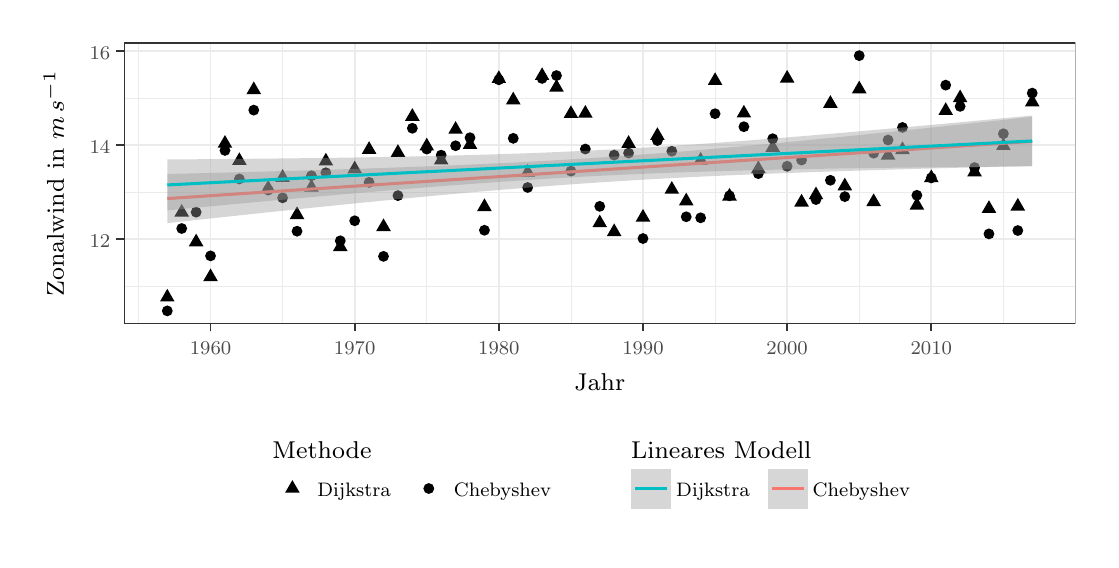
\begin{tikzpicture}[font=\footnotesize,x=1pt,y=1pt]
\definecolor{fillColor}{RGB}{255,255,255}
\path[use as bounding box,fill=fillColor,fill opacity=0.00] (0,0) rectangle (384.11,184.94);
\begin{scope}
\path[clip] (  0.00,  0.00) rectangle (384.11,184.94);
\definecolor{drawColor}{RGB}{255,255,255}
\definecolor{fillColor}{RGB}{255,255,255}

\path[draw=drawColor,line width= 0.6pt,line join=round,line cap=round,fill=fillColor] (  0.00,  0.00) rectangle (384.11,184.94);
\end{scope}
\begin{scope}
\path[clip] ( 34.82, 77.99) rectangle (378.61,179.44);
\definecolor{fillColor}{RGB}{255,255,255}

\path[fill=fillColor] ( 34.82, 77.99) rectangle (378.61,179.44);
\definecolor{drawColor}{gray}{0.92}

\path[draw=drawColor,line width= 0.3pt,line join=round] ( 34.82, 91.45) --
	(378.61, 91.45);

\path[draw=drawColor,line width= 0.3pt,line join=round] ( 34.82,125.46) --
	(378.61,125.46);

\path[draw=drawColor,line width= 0.3pt,line join=round] ( 34.82,159.47) --
	(378.61,159.47);

\path[draw=drawColor,line width= 0.3pt,line join=round] ( 40.03, 77.99) --
	( 40.03,179.44);

\path[draw=drawColor,line width= 0.3pt,line join=round] ( 92.12, 77.99) --
	( 92.12,179.44);

\path[draw=drawColor,line width= 0.3pt,line join=round] (144.21, 77.99) --
	(144.21,179.44);

\path[draw=drawColor,line width= 0.3pt,line join=round] (196.30, 77.99) --
	(196.30,179.44);

\path[draw=drawColor,line width= 0.3pt,line join=round] (248.39, 77.99) --
	(248.39,179.44);

\path[draw=drawColor,line width= 0.3pt,line join=round] (300.48, 77.99) --
	(300.48,179.44);

\path[draw=drawColor,line width= 0.3pt,line join=round] (352.57, 77.99) --
	(352.57,179.44);

\path[draw=drawColor,line width= 0.3pt,line join=round] (378.61, 77.99) --
	(378.61,179.44);

\path[draw=drawColor,line width= 0.6pt,line join=round] ( 34.82,108.46) --
	(378.61,108.46);

\path[draw=drawColor,line width= 0.6pt,line join=round] ( 34.82,142.47) --
	(378.61,142.47);

\path[draw=drawColor,line width= 0.6pt,line join=round] ( 34.82,176.47) --
	(378.61,176.47);

\path[draw=drawColor,line width= 0.6pt,line join=round] ( 66.08, 77.99) --
	( 66.08,179.44);

\path[draw=drawColor,line width= 0.6pt,line join=round] (118.17, 77.99) --
	(118.17,179.44);

\path[draw=drawColor,line width= 0.6pt,line join=round] (170.26, 77.99) --
	(170.26,179.44);

\path[draw=drawColor,line width= 0.6pt,line join=round] (222.34, 77.99) --
	(222.34,179.44);

\path[draw=drawColor,line width= 0.6pt,line join=round] (274.43, 77.99) --
	(274.43,179.44);

\path[draw=drawColor,line width= 0.6pt,line join=round] (326.52, 77.99) --
	(326.52,179.44);
\definecolor{fillColor}{RGB}{0,0,0}

\path[fill=fillColor] ( 50.45, 82.60) circle (  1.96);

\path[fill=fillColor] ( 55.66,112.37) circle (  1.96);

\path[fill=fillColor] ( 60.87,118.27) circle (  1.96);

\path[fill=fillColor] ( 66.08,102.47) circle (  1.96);

\path[fill=fillColor] ( 71.29,140.58) circle (  1.96);

\path[fill=fillColor] ( 76.49,130.27) circle (  1.96);

\path[fill=fillColor] ( 81.70,155.14) circle (  1.96);

\path[fill=fillColor] ( 86.91,126.25) circle (  1.96);

\path[fill=fillColor] ( 92.12,123.46) circle (  1.96);

\path[fill=fillColor] ( 97.33,111.39) circle (  1.96);

\path[fill=fillColor] (102.54,131.43) circle (  1.96);

\path[fill=fillColor] (107.75,132.51) circle (  1.96);

\path[fill=fillColor] (112.96,107.92) circle (  1.96);

\path[fill=fillColor] (118.17,115.16) circle (  1.96);

\path[fill=fillColor] (123.37,129.04) circle (  1.96);

\path[fill=fillColor] (128.58,102.30) circle (  1.96);

\path[fill=fillColor] (133.79,124.25) circle (  1.96);

\path[fill=fillColor] (139.00,148.59) circle (  1.96);

\path[fill=fillColor] (144.21,141.07) circle (  1.96);

\path[fill=fillColor] (149.42,138.87) circle (  1.96);

\path[fill=fillColor] (154.63,142.27) circle (  1.96);

\path[fill=fillColor] (159.84,145.18) circle (  1.96);

\path[fill=fillColor] (165.05,111.73) circle (  1.96);

\path[fill=fillColor] (170.26,166.11) circle (  1.96);

\path[fill=fillColor] (175.46,144.95) circle (  1.96);

\path[fill=fillColor] (180.67,127.19) circle (  1.96);

\path[fill=fillColor] (185.88,166.60) circle (  1.96);

\path[fill=fillColor] (191.09,167.63) circle (  1.96);

\path[fill=fillColor] (196.30,133.11) circle (  1.96);

\path[fill=fillColor] (201.51,141.09) circle (  1.96);

\path[fill=fillColor] (206.72,120.37) circle (  1.96);

\path[fill=fillColor] (211.93,138.88) circle (  1.96);

\path[fill=fillColor] (217.14,139.62) circle (  1.96);

\path[fill=fillColor] (222.34,108.74) circle (  1.96);

\path[fill=fillColor] (227.55,144.15) circle (  1.96);

\path[fill=fillColor] (232.76,140.29) circle (  1.96);

\path[fill=fillColor] (237.97,116.61) circle (  1.96);

\path[fill=fillColor] (243.18,116.23) circle (  1.96);

\path[fill=fillColor] (248.39,153.85) circle (  1.96);

\path[fill=fillColor] (253.60,124.19) circle (  1.96);

\path[fill=fillColor] (258.81,149.15) circle (  1.96);

\path[fill=fillColor] (264.02,132.19) circle (  1.96);

\path[fill=fillColor] (269.22,144.81) circle (  1.96);

\path[fill=fillColor] (274.43,134.85) circle (  1.96);

\path[fill=fillColor] (279.64,137.11) circle (  1.96);

\path[fill=fillColor] (284.85,122.83) circle (  1.96);

\path[fill=fillColor] (290.06,129.79) circle (  1.96);

\path[fill=fillColor] (295.27,123.89) circle (  1.96);

\path[fill=fillColor] (300.48,174.83) circle (  1.96);

\path[fill=fillColor] (305.69,139.59) circle (  1.96);

\path[fill=fillColor] (310.90,144.33) circle (  1.96);

\path[fill=fillColor] (316.11,148.88) circle (  1.96);

\path[fill=fillColor] (321.31,124.37) circle (  1.96);

\path[fill=fillColor] (326.52,130.65) circle (  1.96);

\path[fill=fillColor] (331.73,164.17) circle (  1.96);

\path[fill=fillColor] (336.94,156.50) circle (  1.96);

\path[fill=fillColor] (342.15,134.39) circle (  1.96);

\path[fill=fillColor] (347.36,110.42) circle (  1.96);

\path[fill=fillColor] (352.57,146.61) circle (  1.96);

\path[fill=fillColor] (357.78,111.63) circle (  1.96);

\path[fill=fillColor] (362.99,161.29) circle (  1.96);

\path[fill=fillColor] ( 50.45, 90.57) --
	( 53.09, 86.00) --
	( 47.81, 86.00) --
	cycle;

\path[fill=fillColor] ( 55.66,121.25) --
	( 58.30,116.68) --
	( 53.02,116.68) --
	cycle;

\path[fill=fillColor] ( 60.87,110.52) --
	( 63.51,105.95) --
	( 58.23,105.95) --
	cycle;

\path[fill=fillColor] ( 66.08, 97.93) --
	( 68.72, 93.35) --
	( 63.43, 93.35) --
	cycle;

\path[fill=fillColor] ( 71.29,146.13) --
	( 73.93,141.56) --
	( 68.64,141.56) --
	cycle;

\path[fill=fillColor] ( 76.49,139.90) --
	( 79.14,135.32) --
	( 73.85,135.32) --
	cycle;

\path[fill=fillColor] ( 81.70,165.52) --
	( 84.35,160.95) --
	( 79.06,160.95) --
	cycle;

\path[fill=fillColor] ( 86.91,129.88) --
	( 89.56,125.31) --
	( 84.27,125.31) --
	cycle;

\path[fill=fillColor] ( 92.12,133.82) --
	( 94.76,129.24) --
	( 89.48,129.24) --
	cycle;

\path[fill=fillColor] ( 97.33,120.36) --
	( 99.97,115.79) --
	( 94.69,115.79) --
	cycle;

\path[fill=fillColor] (102.54,130.23) --
	(105.18,125.66) --
	( 99.90,125.66) --
	cycle;

\path[fill=fillColor] (107.75,139.73) --
	(110.39,135.15) --
	(105.11,135.15) --
	cycle;

\path[fill=fillColor] (112.96,108.79) --
	(115.60,104.22) --
	(110.31,104.22) --
	cycle;

\path[fill=fillColor] (118.17,136.88) --
	(120.81,132.30) --
	(115.52,132.30) --
	cycle;

\path[fill=fillColor] (123.37,143.92) --
	(126.02,139.35) --
	(120.73,139.35) --
	cycle;

\path[fill=fillColor] (128.58,116.03) --
	(131.23,111.46) --
	(125.94,111.46) --
	cycle;

\path[fill=fillColor] (133.79,142.84) --
	(136.44,138.26) --
	(131.15,138.26) --
	cycle;

\path[fill=fillColor] (139.00,155.88) --
	(141.64,151.30) --
	(136.36,151.30) --
	cycle;

\path[fill=fillColor] (144.21,145.18) --
	(146.85,140.60) --
	(141.57,140.60) --
	cycle;

\path[fill=fillColor] (149.42,140.11) --
	(152.06,135.53) --
	(146.78,135.53) --
	cycle;

\path[fill=fillColor] (154.63,151.19) --
	(157.27,146.61) --
	(151.99,146.61) --
	cycle;

\path[fill=fillColor] (159.84,145.70) --
	(162.48,141.12) --
	(157.19,141.12) --
	cycle;

\path[fill=fillColor] (165.05,123.27) --
	(167.69,118.69) --
	(162.40,118.69) --
	cycle;

\path[fill=fillColor] (170.26,169.55) --
	(172.90,164.97) --
	(167.61,164.97) --
	cycle;

\path[fill=fillColor] (175.46,161.81) --
	(178.11,157.23) --
	(172.82,157.23) --
	cycle;

\path[fill=fillColor] (180.67,135.71) --
	(183.32,131.13) --
	(178.03,131.13) --
	cycle;

\path[fill=fillColor] (185.88,170.61) --
	(188.52,166.03) --
	(183.24,166.03) --
	cycle;

\path[fill=fillColor] (191.09,166.39) --
	(193.73,161.81) --
	(188.45,161.81) --
	cycle;

\path[fill=fillColor] (196.30,156.87) --
	(198.94,152.30) --
	(193.66,152.30) --
	cycle;

\path[fill=fillColor] (201.51,157.00) --
	(204.15,152.42) --
	(198.87,152.42) --
	cycle;

\path[fill=fillColor] (206.72,117.42) --
	(209.36,112.85) --
	(204.08,112.85) --
	cycle;

\path[fill=fillColor] (211.93,114.21) --
	(214.57,109.63) --
	(209.28,109.63) --
	cycle;

\path[fill=fillColor] (217.14,146.12) --
	(219.78,141.54) --
	(214.49,141.54) --
	cycle;

\path[fill=fillColor] (222.34,119.44) --
	(224.99,114.87) --
	(219.70,114.87) --
	cycle;

\path[fill=fillColor] (227.55,148.96) --
	(230.20,144.38) --
	(224.91,144.38) --
	cycle;

\path[fill=fillColor] (232.76,129.52) --
	(235.40,124.94) --
	(230.12,124.94) --
	cycle;

\path[fill=fillColor] (237.97,125.32) --
	(240.61,120.74) --
	(235.33,120.74) --
	cycle;

\path[fill=fillColor] (243.18,140.01) --
	(245.82,135.43) --
	(240.54,135.43) --
	cycle;

\path[fill=fillColor] (248.39,168.83) --
	(251.03,164.25) --
	(245.75,164.25) --
	cycle;

\path[fill=fillColor] (253.60,127.06) --
	(256.24,122.48) --
	(250.96,122.48) --
	cycle;

\path[fill=fillColor] (258.81,157.06) --
	(261.45,152.48) --
	(256.16,152.48) --
	cycle;

\path[fill=fillColor] (264.02,136.96) --
	(266.66,132.38) --
	(261.37,132.38) --
	cycle;

\path[fill=fillColor] (269.22,144.66) --
	(271.87,140.08) --
	(266.58,140.08) --
	cycle;

\path[fill=fillColor] (274.43,169.66) --
	(277.08,165.09) --
	(271.79,165.09) --
	cycle;

\path[fill=fillColor] (279.64,124.89) --
	(282.29,120.31) --
	(277.00,120.31) --
	cycle;

\path[fill=fillColor] (284.85,127.54) --
	(287.49,122.96) --
	(282.21,122.96) --
	cycle;

\path[fill=fillColor] (290.06,160.57) --
	(292.70,155.99) --
	(287.42,155.99) --
	cycle;

\path[fill=fillColor] (295.27,130.76) --
	(297.91,126.19) --
	(292.63,126.19) --
	cycle;

\path[fill=fillColor] (300.48,165.82) --
	(303.12,161.24) --
	(297.84,161.24) --
	cycle;

\path[fill=fillColor] (305.69,125.07) --
	(308.33,120.49) --
	(303.04,120.49) --
	cycle;

\path[fill=fillColor] (310.90,141.87) --
	(313.54,137.29) --
	(308.25,137.29) --
	cycle;

\path[fill=fillColor] (316.11,143.86) --
	(318.75,139.28) --
	(313.46,139.28) --
	cycle;

\path[fill=fillColor] (321.31,123.78) --
	(323.96,119.20) --
	(318.67,119.20) --
	cycle;

\path[fill=fillColor] (326.52,133.72) --
	(329.17,129.14) --
	(323.88,129.14) --
	cycle;

\path[fill=fillColor] (331.73,157.99) --
	(334.37,153.41) --
	(329.09,153.41) --
	cycle;

\path[fill=fillColor] (336.94,162.58) --
	(339.58,158.00) --
	(334.30,158.00) --
	cycle;

\path[fill=fillColor] (342.15,135.80) --
	(344.79,131.23) --
	(339.51,131.23) --
	cycle;

\path[fill=fillColor] (347.36,122.59) --
	(350.00,118.02) --
	(344.72,118.02) --
	cycle;

\path[fill=fillColor] (352.57,145.32) --
	(355.21,140.74) --
	(349.93,140.74) --
	cycle;

\path[fill=fillColor] (357.78,123.44) --
	(360.42,118.87) --
	(355.13,118.87) --
	cycle;

\path[fill=fillColor] (362.99,161.08) --
	(365.63,156.50) --
	(360.34,156.50) --
	cycle;
\definecolor{fillColor}{RGB}{153,153,153}

\path[fill=fillColor,fill opacity=0.40] ( 50.45,132.06) --
	( 54.41,132.15) --
	( 58.36,132.25) --
	( 62.32,132.35) --
	( 66.27,132.45) --
	( 70.23,132.55) --
	( 74.19,132.65) --
	( 78.14,132.75) --
	( 82.10,132.86) --
	( 86.06,132.96) --
	( 90.01,133.07) --
	( 93.97,133.18) --
	( 97.92,133.29) --
	(101.88,133.41) --
	(105.84,133.53) --
	(109.79,133.65) --
	(113.75,133.77) --
	(117.70,133.89) --
	(121.66,134.02) --
	(125.62,134.15) --
	(129.57,134.29) --
	(133.53,134.43) --
	(137.49,134.57) --
	(141.44,134.72) --
	(145.40,134.87) --
	(149.35,135.03) --
	(153.31,135.19) --
	(157.27,135.35) --
	(161.22,135.53) --
	(165.18,135.71) --
	(169.13,135.89) --
	(173.09,136.08) --
	(177.05,136.28) --
	(181.00,136.49) --
	(184.96,136.70) --
	(188.92,136.92) --
	(192.87,137.15) --
	(196.83,137.39) --
	(200.78,137.63) --
	(204.74,137.88) --
	(208.70,138.15) --
	(212.65,138.42) --
	(216.61,138.69) --
	(220.56,138.98) --
	(224.52,139.27) --
	(228.48,139.58) --
	(232.43,139.89) --
	(236.39,140.20) --
	(240.34,140.53) --
	(244.30,140.86) --
	(248.26,141.20) --
	(252.21,141.54) --
	(256.17,141.89) --
	(260.13,142.25) --
	(264.08,142.61) --
	(268.04,142.98) --
	(271.99,143.35) --
	(275.95,143.73) --
	(279.91,144.11) --
	(283.86,144.49) --
	(287.82,144.88) --
	(291.77,145.27) --
	(295.73,145.67) --
	(299.69,146.06) --
	(303.64,146.46) --
	(307.60,146.87) --
	(311.56,147.27) --
	(315.51,147.68) --
	(319.47,148.09) --
	(323.42,148.51) --
	(327.38,148.92) --
	(331.34,149.34) --
	(335.29,149.76) --
	(339.25,150.18) --
	(343.20,150.60) --
	(347.16,151.02) --
	(351.12,151.44) --
	(355.07,151.87) --
	(359.03,152.30) --
	(362.99,152.73) --
	(362.99,134.99) --
	(359.03,134.90) --
	(355.07,134.80) --
	(351.12,134.70) --
	(347.16,134.60) --
	(343.20,134.50) --
	(339.25,134.40) --
	(335.29,134.30) --
	(331.34,134.19) --
	(327.38,134.09) --
	(323.42,133.98) --
	(319.47,133.87) --
	(315.51,133.75) --
	(311.56,133.64) --
	(307.60,133.52) --
	(303.64,133.40) --
	(299.69,133.28) --
	(295.73,133.16) --
	(291.77,133.03) --
	(287.82,132.90) --
	(283.86,132.76) --
	(279.91,132.62) --
	(275.95,132.48) --
	(271.99,132.33) --
	(268.04,132.18) --
	(264.08,132.02) --
	(260.13,131.86) --
	(256.17,131.70) --
	(252.21,131.52) --
	(248.26,131.34) --
	(244.30,131.16) --
	(240.34,130.97) --
	(236.39,130.77) --
	(232.43,130.56) --
	(228.48,130.35) --
	(224.52,130.13) --
	(220.56,129.90) --
	(216.61,129.66) --
	(212.65,129.42) --
	(208.70,129.17) --
	(204.74,128.90) --
	(200.78,128.63) --
	(196.83,128.36) --
	(192.87,128.07) --
	(188.92,127.78) --
	(184.96,127.47) --
	(181.00,127.16) --
	(177.05,126.85) --
	(173.09,126.52) --
	(169.13,126.19) --
	(165.18,125.85) --
	(161.22,125.51) --
	(157.27,125.16) --
	(153.31,124.80) --
	(149.35,124.44) --
	(145.40,124.07) --
	(141.44,123.70) --
	(137.49,123.32) --
	(133.53,122.94) --
	(129.57,122.56) --
	(125.62,122.17) --
	(121.66,121.78) --
	(117.70,121.38) --
	(113.75,120.99) --
	(109.79,120.59) --
	(105.84,120.18) --
	(101.88,119.78) --
	( 97.92,119.37) --
	( 93.97,118.96) --
	( 90.01,118.54) --
	( 86.06,118.13) --
	( 82.10,117.71) --
	( 78.14,117.29) --
	( 74.19,116.87) --
	( 70.23,116.45) --
	( 66.27,116.03) --
	( 62.32,115.60) --
	( 58.36,115.18) --
	( 54.41,114.75) --
	( 50.45,114.32) --
	cycle;
\definecolor{drawColor}{RGB}{248,118,109}

\path[draw=drawColor,line width= 1.1pt,line join=round] ( 50.45,123.19) --
	( 54.41,123.45) --
	( 58.36,123.71) --
	( 62.32,123.98) --
	( 66.27,124.24) --
	( 70.23,124.50) --
	( 74.19,124.76) --
	( 78.14,125.02) --
	( 82.10,125.28) --
	( 86.06,125.55) --
	( 90.01,125.81) --
	( 93.97,126.07) --
	( 97.92,126.33) --
	(101.88,126.59) --
	(105.84,126.85) --
	(109.79,127.12) --
	(113.75,127.38) --
	(117.70,127.64) --
	(121.66,127.90) --
	(125.62,128.16) --
	(129.57,128.42) --
	(133.53,128.69) --
	(137.49,128.95) --
	(141.44,129.21) --
	(145.40,129.47) --
	(149.35,129.73) --
	(153.31,129.99) --
	(157.27,130.25) --
	(161.22,130.52) --
	(165.18,130.78) --
	(169.13,131.04) --
	(173.09,131.30) --
	(177.05,131.56) --
	(181.00,131.82) --
	(184.96,132.09) --
	(188.92,132.35) --
	(192.87,132.61) --
	(196.83,132.87) --
	(200.78,133.13) --
	(204.74,133.39) --
	(208.70,133.66) --
	(212.65,133.92) --
	(216.61,134.18) --
	(220.56,134.44) --
	(224.52,134.70) --
	(228.48,134.96) --
	(232.43,135.23) --
	(236.39,135.49) --
	(240.34,135.75) --
	(244.30,136.01) --
	(248.26,136.27) --
	(252.21,136.53) --
	(256.17,136.79) --
	(260.13,137.06) --
	(264.08,137.32) --
	(268.04,137.58) --
	(271.99,137.84) --
	(275.95,138.10) --
	(279.91,138.36) --
	(283.86,138.63) --
	(287.82,138.89) --
	(291.77,139.15) --
	(295.73,139.41) --
	(299.69,139.67) --
	(303.64,139.93) --
	(307.60,140.20) --
	(311.56,140.46) --
	(315.51,140.72) --
	(319.47,140.98) --
	(323.42,141.24) --
	(327.38,141.50) --
	(331.34,141.77) --
	(335.29,142.03) --
	(339.25,142.29) --
	(343.20,142.55) --
	(347.16,142.81) --
	(351.12,143.07) --
	(355.07,143.33) --
	(359.03,143.60) --
	(362.99,143.86);

\path[fill=fillColor,fill opacity=0.40] ( 50.45,137.31) --
	( 54.41,137.34) --
	( 58.36,137.37) --
	( 62.32,137.40) --
	( 66.27,137.43) --
	( 70.23,137.47) --
	( 74.19,137.50) --
	( 78.14,137.54) --
	( 82.10,137.58) --
	( 86.06,137.62) --
	( 90.01,137.66) --
	( 93.97,137.70) --
	( 97.92,137.75) --
	(101.88,137.80) --
	(105.84,137.85) --
	(109.79,137.90) --
	(113.75,137.96) --
	(117.70,138.02) --
	(121.66,138.08) --
	(125.62,138.15) --
	(129.57,138.22) --
	(133.53,138.29) --
	(137.49,138.37) --
	(141.44,138.45) --
	(145.40,138.54) --
	(149.35,138.63) --
	(153.31,138.73) --
	(157.27,138.83) --
	(161.22,138.94) --
	(165.18,139.06) --
	(169.13,139.18) --
	(173.09,139.31) --
	(177.05,139.44) --
	(181.00,139.58) --
	(184.96,139.73) --
	(188.92,139.89) --
	(192.87,140.06) --
	(196.83,140.24) --
	(200.78,140.42) --
	(204.74,140.61) --
	(208.70,140.81) --
	(212.65,141.02) --
	(216.61,141.24) --
	(220.56,141.47) --
	(224.52,141.70) --
	(228.48,141.95) --
	(232.43,142.20) --
	(236.39,142.46) --
	(240.34,142.72) --
	(244.30,143.00) --
	(248.26,143.28) --
	(252.21,143.56) --
	(256.17,143.86) --
	(260.13,144.16) --
	(264.08,144.46) --
	(268.04,144.77) --
	(271.99,145.09) --
	(275.95,145.41) --
	(279.91,145.73) --
	(283.86,146.06) --
	(287.82,146.39) --
	(291.77,146.73) --
	(295.73,147.07) --
	(299.69,147.41) --
	(303.64,147.76) --
	(307.60,148.10) --
	(311.56,148.46) --
	(315.51,148.81) --
	(319.47,149.16) --
	(323.42,149.52) --
	(327.38,149.88) --
	(331.34,150.24) --
	(335.29,150.61) --
	(339.25,150.97) --
	(343.20,151.34) --
	(347.16,151.71) --
	(351.12,152.08) --
	(355.07,152.45) --
	(359.03,152.82) --
	(362.99,153.20) --
	(362.99,134.80) --
	(359.03,134.77) --
	(355.07,134.74) --
	(351.12,134.71) --
	(347.16,134.68) --
	(343.20,134.64) --
	(339.25,134.61) --
	(335.29,134.57) --
	(331.34,134.53) --
	(327.38,134.49) --
	(323.42,134.45) --
	(319.47,134.41) --
	(315.51,134.36) --
	(311.56,134.31) --
	(307.60,134.26) --
	(303.64,134.21) --
	(299.69,134.15) --
	(295.73,134.09) --
	(291.77,134.03) --
	(287.82,133.96) --
	(283.86,133.89) --
	(279.91,133.82) --
	(275.95,133.74) --
	(271.99,133.66) --
	(268.04,133.57) --
	(264.08,133.48) --
	(260.13,133.38) --
	(256.17,133.28) --
	(252.21,133.17) --
	(248.26,133.05) --
	(244.30,132.93) --
	(240.34,132.80) --
	(236.39,132.67) --
	(232.43,132.53) --
	(228.48,132.38) --
	(224.52,132.22) --
	(220.56,132.05) --
	(216.61,131.87) --
	(212.65,131.69) --
	(208.70,131.50) --
	(204.74,131.30) --
	(200.78,131.09) --
	(196.83,130.87) --
	(192.87,130.64) --
	(188.92,130.41) --
	(184.96,130.16) --
	(181.00,129.91) --
	(177.05,129.65) --
	(173.09,129.39) --
	(169.13,129.11) --
	(165.18,128.83) --
	(161.22,128.55) --
	(157.27,128.25) --
	(153.31,127.95) --
	(149.35,127.65) --
	(145.40,127.34) --
	(141.44,127.02) --
	(137.49,126.70) --
	(133.53,126.38) --
	(129.57,126.05) --
	(125.62,125.72) --
	(121.66,125.38) --
	(117.70,125.04) --
	(113.75,124.70) --
	(109.79,124.35) --
	(105.84,124.01) --
	(101.88,123.65) --
	( 97.92,123.30) --
	( 93.97,122.95) --
	( 90.01,122.59) --
	( 86.06,122.23) --
	( 82.10,121.87) --
	( 78.14,121.50) --
	( 74.19,121.14) --
	( 70.23,120.77) --
	( 66.27,120.40) --
	( 62.32,120.03) --
	( 58.36,119.66) --
	( 54.41,119.29) --
	( 50.45,118.91) --
	cycle;
\definecolor{drawColor}{RGB}{0,191,196}

\path[draw=drawColor,line width= 1.1pt,line join=round] ( 50.45,128.11) --
	( 54.41,128.31) --
	( 58.36,128.51) --
	( 62.32,128.72) --
	( 66.27,128.92) --
	( 70.23,129.12) --
	( 74.19,129.32) --
	( 78.14,129.52) --
	( 82.10,129.72) --
	( 86.06,129.92) --
	( 90.01,130.12) --
	( 93.97,130.32) --
	( 97.92,130.53) --
	(101.88,130.73) --
	(105.84,130.93) --
	(109.79,131.13) --
	(113.75,131.33) --
	(117.70,131.53) --
	(121.66,131.73) --
	(125.62,131.93) --
	(129.57,132.13) --
	(133.53,132.34) --
	(137.49,132.54) --
	(141.44,132.74) --
	(145.40,132.94) --
	(149.35,133.14) --
	(153.31,133.34) --
	(157.27,133.54) --
	(161.22,133.74) --
	(165.18,133.94) --
	(169.13,134.14) --
	(173.09,134.35) --
	(177.05,134.55) --
	(181.00,134.75) --
	(184.96,134.95) --
	(188.92,135.15) --
	(192.87,135.35) --
	(196.83,135.55) --
	(200.78,135.75) --
	(204.74,135.95) --
	(208.70,136.16) --
	(212.65,136.36) --
	(216.61,136.56) --
	(220.56,136.76) --
	(224.52,136.96) --
	(228.48,137.16) --
	(232.43,137.36) --
	(236.39,137.56) --
	(240.34,137.76) --
	(244.30,137.97) --
	(248.26,138.17) --
	(252.21,138.37) --
	(256.17,138.57) --
	(260.13,138.77) --
	(264.08,138.97) --
	(268.04,139.17) --
	(271.99,139.37) --
	(275.95,139.57) --
	(279.91,139.77) --
	(283.86,139.98) --
	(287.82,140.18) --
	(291.77,140.38) --
	(295.73,140.58) --
	(299.69,140.78) --
	(303.64,140.98) --
	(307.60,141.18) --
	(311.56,141.38) --
	(315.51,141.58) --
	(319.47,141.79) --
	(323.42,141.99) --
	(327.38,142.19) --
	(331.34,142.39) --
	(335.29,142.59) --
	(339.25,142.79) --
	(343.20,142.99) --
	(347.16,143.19) --
	(351.12,143.39) --
	(355.07,143.60) --
	(359.03,143.80) --
	(362.99,144.00);
\definecolor{drawColor}{gray}{0.20}

\path[draw=drawColor,line width= 0.6pt,line join=round,line cap=round] ( 34.82, 77.99) rectangle (378.61,179.44);
\end{scope}
\begin{scope}
\path[clip] (  0.00,  0.00) rectangle (384.11,184.94);
\definecolor{drawColor}{gray}{0.30}

\node[text=drawColor,anchor=base east,inner sep=0pt, outer sep=0pt, scale=  0.88] at ( 29.87,105.43) {12};

\node[text=drawColor,anchor=base east,inner sep=0pt, outer sep=0pt, scale=  0.88] at ( 29.87,139.44) {14};

\node[text=drawColor,anchor=base east,inner sep=0pt, outer sep=0pt, scale=  0.88] at ( 29.87,173.44) {16};
\end{scope}
\begin{scope}
\path[clip] (  0.00,  0.00) rectangle (384.11,184.94);
\definecolor{drawColor}{gray}{0.20}

\path[draw=drawColor,line width= 0.6pt,line join=round] ( 32.07,108.46) --
	( 34.82,108.46);

\path[draw=drawColor,line width= 0.6pt,line join=round] ( 32.07,142.47) --
	( 34.82,142.47);

\path[draw=drawColor,line width= 0.6pt,line join=round] ( 32.07,176.47) --
	( 34.82,176.47);
\end{scope}
\begin{scope}
\path[clip] (  0.00,  0.00) rectangle (384.11,184.94);
\definecolor{drawColor}{gray}{0.20}

\path[draw=drawColor,line width= 0.6pt,line join=round] ( 66.08, 75.24) --
	( 66.08, 77.99);

\path[draw=drawColor,line width= 0.6pt,line join=round] (118.17, 75.24) --
	(118.17, 77.99);

\path[draw=drawColor,line width= 0.6pt,line join=round] (170.26, 75.24) --
	(170.26, 77.99);

\path[draw=drawColor,line width= 0.6pt,line join=round] (222.34, 75.24) --
	(222.34, 77.99);

\path[draw=drawColor,line width= 0.6pt,line join=round] (274.43, 75.24) --
	(274.43, 77.99);

\path[draw=drawColor,line width= 0.6pt,line join=round] (326.52, 75.24) --
	(326.52, 77.99);
\end{scope}
\begin{scope}
\path[clip] (  0.00,  0.00) rectangle (384.11,184.94);
\definecolor{drawColor}{gray}{0.30}

\node[text=drawColor,anchor=base,inner sep=0pt, outer sep=0pt, scale=  0.88] at ( 66.08, 66.98) {1960};

\node[text=drawColor,anchor=base,inner sep=0pt, outer sep=0pt, scale=  0.88] at (118.17, 66.98) {1970};

\node[text=drawColor,anchor=base,inner sep=0pt, outer sep=0pt, scale=  0.88] at (170.26, 66.98) {1980};

\node[text=drawColor,anchor=base,inner sep=0pt, outer sep=0pt, scale=  0.88] at (222.34, 66.98) {1990};

\node[text=drawColor,anchor=base,inner sep=0pt, outer sep=0pt, scale=  0.88] at (274.43, 66.98) {2000};

\node[text=drawColor,anchor=base,inner sep=0pt, outer sep=0pt, scale=  0.88] at (326.52, 66.98) {2010};
\end{scope}
\begin{scope}
\path[clip] (  0.00,  0.00) rectangle (384.11,184.94);
\definecolor{drawColor}{RGB}{0,0,0}

\node[text=drawColor,anchor=base,inner sep=0pt, outer sep=0pt, scale=  1.10] at (206.72, 53.91) {Jahr};
\end{scope}
\begin{scope}
\path[clip] (  0.00,  0.00) rectangle (384.11,184.94);
\definecolor{drawColor}{RGB}{0,0,0}

\node[text=drawColor,rotate= 90.00,anchor=base,inner sep=0pt, outer sep=0pt, scale=  1.10] at ( 13.08,128.72) {Zonalwind in $m\,s^{-1}$};
\end{scope}
\begin{scope}
\path[clip] (  0.00,  0.00) rectangle (384.11,184.94);
\definecolor{fillColor}{RGB}{255,255,255}

\path[fill=fillColor] ( 82.74,  5.50) rectangle (201.03, 42.52);
\end{scope}
\begin{scope}
\path[clip] (  0.00,  0.00) rectangle (384.11,184.94);
\definecolor{drawColor}{RGB}{0,0,0}

\node[text=drawColor,anchor=base west,inner sep=0pt, outer sep=0pt, scale=  1.10] at ( 88.43, 29.26) {Methode};
\end{scope}
\begin{scope}
\path[clip] (  0.00,  0.00) rectangle (384.11,184.94);
\definecolor{fillColor}{RGB}{255,255,255}

\path[fill=fillColor] ( 88.43, 11.19) rectangle (102.88, 25.64);
\end{scope}
\begin{scope}
\path[clip] (  0.00,  0.00) rectangle (384.11,184.94);
\definecolor{fillColor}{RGB}{0,0,0}

\path[fill=fillColor] ( 95.65, 21.47) --
	( 98.30, 16.89) --
	( 93.01, 16.89) --
	cycle;
\end{scope}
\begin{scope}
\path[clip] (  0.00,  0.00) rectangle (384.11,184.94);
\definecolor{fillColor}{RGB}{255,255,255}

\path[fill=fillColor] (137.73, 11.19) rectangle (152.18, 25.64);
\end{scope}
\begin{scope}
\path[clip] (  0.00,  0.00) rectangle (384.11,184.94);
\definecolor{fillColor}{RGB}{0,0,0}

\path[fill=fillColor] (144.95, 18.42) circle (  1.96);
\end{scope}
\begin{scope}
\path[clip] (  0.00,  0.00) rectangle (384.11,184.94);
\definecolor{drawColor}{RGB}{0,0,0}

\node[text=drawColor,anchor=base west,inner sep=0pt, outer sep=0pt, scale=  0.88] at (104.69, 15.39) {Dijkstra};
\end{scope}
\begin{scope}
\path[clip] (  0.00,  0.00) rectangle (384.11,184.94);
\definecolor{drawColor}{RGB}{0,0,0}

\node[text=drawColor,anchor=base west,inner sep=0pt, outer sep=0pt, scale=  0.88] at (153.99, 15.39) {Chebyshev};
\end{scope}
\begin{scope}
\path[clip] (  0.00,  0.00) rectangle (384.11,184.94);
\definecolor{fillColor}{RGB}{255,255,255}

\path[fill=fillColor] (212.41,  5.50) rectangle (330.70, 42.52);
\end{scope}
\begin{scope}
\path[clip] (  0.00,  0.00) rectangle (384.11,184.94);
\definecolor{drawColor}{RGB}{0,0,0}

\node[text=drawColor,anchor=base west,inner sep=0pt, outer sep=0pt, scale=  1.10] at (218.10, 29.26) {Lineares Modell};
\end{scope}
\begin{scope}
\path[clip] (  0.00,  0.00) rectangle (384.11,184.94);
\definecolor{fillColor}{RGB}{255,255,255}

\path[fill=fillColor] (218.10, 11.19) rectangle (232.55, 25.64);
\end{scope}
\begin{scope}
\path[clip] (  0.00,  0.00) rectangle (384.11,184.94);
\definecolor{fillColor}{RGB}{153,153,153}

\path[fill=fillColor,fill opacity=0.40] (218.10, 11.19) rectangle (232.55, 25.64);
\definecolor{drawColor}{RGB}{0,191,196}

\path[draw=drawColor,line width= 1.1pt,line join=round] (219.54, 18.42) -- (231.11, 18.42);
\end{scope}
\begin{scope}
\path[clip] (  0.00,  0.00) rectangle (384.11,184.94);
\definecolor{fillColor}{RGB}{255,255,255}

\path[fill=fillColor] (267.40, 11.19) rectangle (281.85, 25.64);
\end{scope}
\begin{scope}
\path[clip] (  0.00,  0.00) rectangle (384.11,184.94);
\definecolor{fillColor}{RGB}{153,153,153}

\path[fill=fillColor,fill opacity=0.40] (267.40, 11.19) rectangle (281.85, 25.64);
\definecolor{drawColor}{RGB}{248,118,109}

\path[draw=drawColor,line width= 1.1pt,line join=round] (268.84, 18.42) -- (280.41, 18.42);
\end{scope}
\begin{scope}
\path[clip] (  0.00,  0.00) rectangle (384.11,184.94);
\definecolor{drawColor}{RGB}{0,0,0}

\node[text=drawColor,anchor=base west,inner sep=0pt, outer sep=0pt, scale=  0.88] at (234.36, 15.39) {Dijkstra};
\end{scope}
\begin{scope}
\path[clip] (  0.00,  0.00) rectangle (384.11,184.94);
\definecolor{drawColor}{RGB}{0,0,0}

\node[text=drawColor,anchor=base west,inner sep=0pt, outer sep=0pt, scale=  0.88] at (283.66, 15.39) {Chebyshev};
\end{scope}
\end{tikzpicture}
